\section{Introduction - Functional Programming & Haskell } 
\frame{\sectionpage}



\subsection{Functional Programming}

\begin{frame}\frametitle{Functional Programming} 
		
		\begin{columns}[T] % align columns
			\begin{column}{.72\textwidth}
				\begin{block}{Definition and Intuitive idea}
				\begin{itemize}
					  \item Computation is just \textbf{function evaluation} $\neq$ \textbf{program
					  state manipulation}.
					  \item Based on $\lambda-$calculus that is an alternative (to set theory)
					  and convenient formalization of logic and mathematics for expressing
					  \textbf{computation}
					  \item Logic deduction $\Leftrightarrow$ $\lambda-$calculus thanks to the
					  Curry-Howard correnspondence.
					  \item A program is a proof!
				\end{itemize}
				\end{block}

			\end{column}%
				\hfill%
				\begin{column}{.28\textwidth}
				\begin{figure}
					\centering
					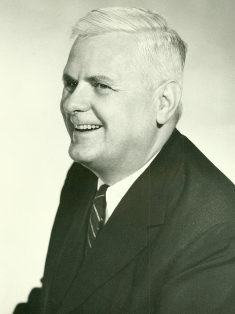
\includegraphics[scale=0.5]{images/Alonzo_Church.jpg}
					\caption{Alonzo-Church, father of $\lambda-$calculus}
				\end{figure}
			\end{column}%
		\end{columns}
	\end{frame}

\begin{frame}[fragile]\frametitle{Imperative vs Functional} 
		\begin{itemize}
		\item Imperative
		  \begin{itemize}
		    \item Focus on low-level \textbf{how}!
		    \item A program is an ordered sequence of instructions
		    \item Modifies/track the program's state
		\end{itemize}
	\end{itemize}
	
	\begin{itemize}
		\item Functional
		  \begin{itemize}
		    \item Focus on High level \textbf{what}!
		    \item Specify high-level transformation/constraint on the desidered result
		    description.
		\end{itemize}
	\end{itemize}
	
	\begin{columns}[T] % align columns
			\begin{column}{.7\textwidth}
				\begin{block}{Imperative, suffer from the so called \textbf{indexitis}}
				\begin{lstlisting}[language=c]
					unsigned int sum=0;
					for(int i=1;i<100;i++)
						 sum+=i;
				\end{lstlisting}
				\end{block}

			\end{column}%
				\hfill%
				\begin{column}{.28\textwidth}
				\begin{block}{Functional}
				\begin{lstlisting}[language=haskell]
					sum [1..99]
				\end{lstlisting}
				\end{block}
			\end{column}%
		\end{columns}
	\end{frame}
	
	
\begin{frame}[fragile]\frametitle{What does this code do?} 
\centering
\begin{lstlisting}[language=c,basicstyle=\footnotesize\ttfamily]
	void function (int *a, int n) {
	    int i, j, p, t;
	    if (n < 2)
	        return;
	    p = a[n / 2];
	    for (i = 0, j = n - 1;; i++, j--) {
	        while (a[i] < p)
	            i++;
	        while (p < a[j])
	            j--;
	        if (i >= j)
	            break;
	        t = a[i];
	        a[i] = a[j];
	        a[j] = t;
	    }
	    function(a, i);
	    function(a + i, n - i);
	}
\end{lstlisting}
\end{frame}	

\begin{frame}[fragile]\frametitle{\ldots and this?} 
\centering
\hline \hfill \\
\begin{lstlisting}[language=haskell,basicstyle=\footnotesize\ttfamily]
function ::(Ord a) =>  [a] -> [a]
function [] = []
function (x:xs) = (function l) ++ [x] ++ (function g)
   where 
	    l = filter (<x) xs
	    g = filter (>=x) xs
\end{lstlisting}
\hline
	\begin{itemize}
	  \item No indices
	  \item No memory/pointer management
	  \item No variable assignment
	\end{itemize}	
\end{frame}	
	
\begin{frame}\frametitle{Imperative vs Functional} 
\begin{table}[h]
\centering
\resizebox{\textwidth}{!}{%
\begin{tabular}{|l|l|l|}
\hline
\textbf{Characteristic}                     & \textbf{Imperative}                        & \textbf{Functional}                                                                            \\ \hline
\textit{\textbf{Programmer focus}}          & Algorithm design                           & What the output look like?                                                                     \\ \hline
\textit{\textbf{State changes}}             & {\color[HTML]{9A0000} Fundamental}         & {\color[HTML]{9A0000} Non-existent}                                                            \\ \hline
\textit{\textbf{Order of execution}}        & Important                                  & \begin{tabular}[c]{@{}l@{}}Low importance\\  (compilers may do much work on this)\end{tabular} \\ \hline
\textit{\textbf{Primary flow control}}      & {\color[HTML]{9A0000} Loops, conditionals} & {\color[HTML]{9A0000} Recursion and Functions}                                                 \\ \hline
\textit{\textbf{Primary data unit}} & structures or classes       
& Functions                                                                                      \\ \hline
\end{tabular}
}
\end{table}

\begin{itemize}
  \item Other pure/quasi-pure languages: Erlang, Scala, F#, LISP.  
\end{itemize}

\end{frame}

\begin{frame}\frametitle{Why Functional Programming? Why Haskell?} 
		\begin{enumerate}
		  \item Haskell's expressive power can improve
		  productivity/understandability/maintanibility
				\begin{itemize}
			    \item Get best from compiled and interpreted languages
			    \item Can understand what complex library does
			  \end{itemize}
		\item Strong typed - Catches bugs at \emph{compile time}
		\item Powerful type inference engine
		\item New Testing metologies
		\item Automatic parallelization due to code purity
		\end{enumerate}
	\end{frame}
	
	\subsection{Tools and Installation}
		\begin{frame}[fragile]\frametitle{Haskell platform}
		A full comprehensive, development environment for
		Haskell\footnote{https://www.haskell.org/platform/index.html}\footnote{http://tryhaskell.org/}.
		
			\begin{block}{Installation}
			\begin{itemize}
			  \item 
				\begin{lstlisting}[language=bash]
					$sudo apt-get install haskell-platform
				\end{lstlisting}
			\end{itemize}
			\end{block}
			
			\begin{description}
			  \item[GHC]
			  	 (Great Glasgow Compiler): State of the art
			  \item[GHCi]
			  	 A read-eval-print loop interpreter
			  \item[Cabal]
			   	Build/distribuite/retrieve libraries
			  \item[Haddock]
			   		A high quality documentation generation tool for Haskell 
			\end{description}
\end{frame}

	\begin{frame}[fragile]\frametitle{What really is Haskell?}
		\begin{block}{Purely Functional language}
			\begin{itemize}
			  \item Functions are first-class object (same things as data)
			\item Deterministic - No Side Effect- same function call $\Rightarrow$ same
			Ouput, EVER!\\
			This \emph{referial transparency} leaves room for compiler optimization and 
			allow to mathematically prove correctness.
			\item safely replace expressions by its (unique) result value
			\item \textbf{Evaluate expression} rather than execute instruction
			\item Function describes what data are, not what what to do to\ldots
			\item Everything (variables, data structures\ldots) is immutable 
			\item Multi-parameters function simply does not exists.
			\end{itemize}
			
		\end{block} 
	
	\end{frame}
	
	\begin{frame}[fragile]\frametitle{Haskell is Lazy}
			\begin{columns}[T] % align columns
			\begin{column}{.67\textwidth}

			\begin{alertblock}{It won't execute anything until is \emph{really
			needed}} 
					\begin{itemize}
					  	\item It is possible to define and work with infinite data structures
					  \item Define new control structure just by defining a function.
					  \item Reasoning about time/space complexity much more complicated
					\end{itemize}
			\end{alertblock}
			

			\end{column}%
			\hfill%
			\begin{column}{.45\textwidth}
			
\includegraphics[scale=0.5]{./images/homer}
			\end{column}%
			\end{columns}
			
			
	\end{frame}
	
	
	
\begin{frame}[fragile]\frametitle{Understanding laziness}
	\begin{lstlisting}[language=Haskell]
		lazyEval 0 b = 1
		lazyEval _ b = b
	\end{lstlisting}
	\begin{itemize}
	  \item b never computed if the first parameter is zero
	  \item this call is safe: 
	  \begin{lstlisting}[language=Haskell] 
	  	lazyEval 0	(2^123123123123123123123)
	  \end{lstlisting}
	  \item this is not 
	    \begin{lstlisting}[language=Haskell] 
	    lazyEval 1 	(2^123123123123123123123)
	  \end{lstlisting}
	\end{itemize}
	\begin{exampleblock}{Strict evaluation: parameter are evaluated
	  \textbf{before} to be passed to functions}
	\begin{itemize}
	 
	\end{itemize}
	
	 	\begin{lstlisting}[language=c++,basicstyle=\footnotesize\ttfamily]
	 	 	int cont=0;
	 	 	auto fcall = [] (int a, int b) 
	 	 	{if(a==0) return 1; else return b;};
	 	 	auto f1 = [] () { cont++; return 1};
	 	 	auto f2 = [] () { cont+=10; return 2};
	    	fcall (f1(),f2()));
	  \end{lstlisting} 
	fcall will always  increments $cont$ twice! 
	\end{exampleblock}
			
			
\end{frame}
	
\subsection{Hello world(s)}
	\begin{frame}[fragile]\frametitle{Hello World}
			\begin{block}{Our First Program}
				Create a file \emph{hello.hs} and compile with the followings
				\begin{lstlisting}[language=Haskell]
						main = putStrLn "Hello World with Haskell"
				\end{lstlisting}
				\begin{lstlisting}[language=bash]
						$ghc -o hello hello.hs
				\end{lstlisting}
			\end{block}
			\begin{block}{GHCi}
				Execute and play with GHCi by simply typing
				\begin{lstlisting}[language=Haskell]
						reverse [1..10]
						:t foldl
						[1..]
						(filter (even) .reverse) [1..100]
				\end{lstlisting}
			\end{block}
		\end{frame}
		
		\begin{frame}[fragile]\frametitle{Hello Currying}
		Another example, the $k^{th}$ Fibonacci number (type in GHCi):
		\begin{lstlisting}[language=Haskell,xleftmargin=-1.5em]
			let f a b k = if k==0 then a else f b (a+b) (k-1)
		\end{lstlisting}
		\begin{itemize}
		  \item	Defines a recursive function \emph{f} that takes \emph{a,b,k} as parameters:
		  \item Spaces are important. Are like function call operator
		  \emph{()} in C-like languages.
		  \item Wait, three space in $f\;a\;b\;k$: 3 function
		  calls? YES!. \textbf{Every function in Haskell officially only takes one
		  parameter}. 
		  \item f infact has type
		 \begin{lstlisting}[language=Haskell,xleftmargin=-1.5em]
			f :: Integer->(Integer->(Integer->Integer))
		\end{lstlisting}
		i.e. a function that takes an integer and return (the \emph{-$>$}) a function
		that takes an integer and return \ldots
		 \begin{lstlisting}[language=Haskell,xleftmargin=-1.5em]
			f 0 :: Integer->(Integer->Integer)
			f 0 1 :: Integer->Integer
			f 0 1 10 :: Integer
		\end{lstlisting}
		
		\end{itemize}
		\end{frame}
		
		\begin{frame}[fragile]\frametitle{Hello Currying - 2}
		Currying directly and naturally address the  high-order functions support
		 Haskell machinery.
		 \begin{alertblock}{High-order function:}
		 \begin{itemize}
		   \item Take function as parameter
		   \item returns a function%\footnote{In haskell \textbf{return exp} has a
		   % different meaning respect to the classic: \textit{return execution of the program to
		   % the caller, and report the valfooue of exp}} 
		\end{itemize}
		 \end{alertblock}
		 
		 \begin{exampleblock}{zipwith}
		  \begin{itemize}
		   \item Combines two list of type $a$ and $b$ using a function f that takes a
		   parameter of type a and one of type b and return a value of type $c$,
		   producing a list of elements of type $c$.
		   \item 
		 \begin{lstlisting}[language=Haskell,xleftmargin=-0.3em]
			zipWith :: (a -> b -> c) -> [a] -> [b] -> [c]
		\end{lstlisting}
		\end{itemize}
		 \end{exampleblock}
		
		
		\end{frame}
		
		
		
		\begin{frame}[fragile]\frametitle{Hello Currying - 2}
		
		\begin{lstlisting}[language=Haskell,xleftmargin=-0.3em]
			zipWith :: (a -> b -> c) -> [a] -> [b] -> [c]
			zipWith _ _ [] = []
			zipWith _ [] _ = []
			zipWith f (x:xs) (y:ys) = f x y : zipWith f xs ys
		\end{lstlisting}
		 \begin{exampleblock}{usage examples}
		  \begin{lstlisting}[language=Haskell,xleftmargin=-0.3em]
			zipWith (+) [1,2,3] [4,5,6] = [5,7,9]
			zipWith (*) [1,2,3] [4,5,6] = [4,10,18]
			zipWith (\a b ->(+).(2*))) [1..] [1..]
		\end{lstlisting}
		What about this call? (missing one parameter)
		\begin{lstlisting}[language=Haskell]
		let l = zipWith (*) [1,2,3] 
		l [3,2,1]
		\end{lstlisting}
		 \end{exampleblock}
		
		\end{frame}
		
		
		
		\begin{frame}[fragile]\frametitle{Hello World - 3}
			
			\begin{exampleblock}{Number of distinct powers counting (Project Euler #29)}
			Consider all integer combinations of $a,b$ for $2 \leq a,b
			\leq 100$:
			how many distinct terms are in the sequence generated by $a^b$?
			\hfill \\
			\begin{smashedalign}
			&2^2=4,2^3=8,\Highlight[blue][blue!20]{$2^4=16$},2^5=32 \\
			&3^2=9,3^3=27,3^4=81,3^5=243\\
			&\Highlight[blue][blue!20]{$4^2=16$},4^3=64,4^4=256,4^5=1024\\
			&5^2=25,5^3=125,5^4=625,5^5=3125\\
			\end{smashedalign}
			\end{exampleblock} \pause
			
			\begin{exampleblock}{Na{\"i}ve solution}
			\begin{lstlisting}[language=Haskell]
			np a b = length $ nub l
				where l = [c^d | c<-[2..a],d<-[2..b]]
		\end{lstlisting}
% 				np :: Integer -> Integer -> Int
% 				np a b = let l = [a^b |a<-[2..a],b<-[2..b]] 
% 					 in length (remDup l)
% 	     		where 
% 	     			remDup = (map  head . group . sort)
			\end{exampleblock}
			
		\end{frame}
	
	
		\begin{frame}[fragile]\frametitle{Statically Typed}
		\begin{itemize}
			  \item Haskell is stricly typed
			  \item Helps in thinking and express program structure
			  \item \textbf{Turns run-time errors into compile-time errors}. 		  
			   “If it compiles, it must be correct” is moslty true\footnote{It is still
			   quite possible to have errors in logic even in a type-correct program}. 
		\end{itemize}
		\begin{block}{Abstraction: Every idea, algorithm, and piece of data should
		occur exactly once in your code.}
		Haskell features as parametric polymorphis, typeclasses high-order functions
		greatly aid in fighting repetition.
		
		\end{block}
			
	\end{frame}
	
		\begin{frame}[fragile]\frametitle{What really is Haskell?}
			\begin{exampleblock}{C-like vs Haskell}
			Code as the one that follows
			\begin{lstlisting}[language=C++]
				int acc = 0;
				for ( int i = 0; i < lst.length; i++ )
 					acc	 = acc + 3 * lst[i];
			\end{lstlisting}
			is full of low-level details of iterating over an array by
			keeping track of a current index. It much elegantely translates in:
			\begin{lstlisting}[language=Haskell]
					sum (map (*3) lst)
			\end{lstlisting}
			\end{exampleblock}
			Other examples:
			\begin{lstlisting}[language=Haskell,xleftmargin=-1.5em]
					partition (even) [49, 58, 76, 82, 83, 90]
					--prime number generation
					let pgen (p:xs) = p : pgen [x|x <- xs, x`mod`p > 0]
					take 40 (pgen [2..])
				\end{lstlisting}
	\end{frame}
	